% Options for packages loaded elsewhere
\PassOptionsToPackage{unicode}{hyperref}
\PassOptionsToPackage{hyphens}{url}
\PassOptionsToPackage{dvipsnames,svgnames,x11names}{xcolor}
%
\documentclass[
  a4paper,
]{article}

\usepackage{amsmath,amssymb}
\usepackage{iftex}
\ifPDFTeX
  \usepackage[T1]{fontenc}
  \usepackage[utf8]{inputenc}
  \usepackage{textcomp} % provide euro and other symbols
\else % if luatex or xetex
  \usepackage{unicode-math}
  \defaultfontfeatures{Scale=MatchLowercase}
  \defaultfontfeatures[\rmfamily]{Ligatures=TeX,Scale=1}
\fi
\usepackage{lmodern}
\ifPDFTeX\else  
    % xetex/luatex font selection
\fi
% Use upquote if available, for straight quotes in verbatim environments
\IfFileExists{upquote.sty}{\usepackage{upquote}}{}
\IfFileExists{microtype.sty}{% use microtype if available
  \usepackage[]{microtype}
  \UseMicrotypeSet[protrusion]{basicmath} % disable protrusion for tt fonts
}{}
\makeatletter
\@ifundefined{KOMAClassName}{% if non-KOMA class
  \IfFileExists{parskip.sty}{%
    \usepackage{parskip}
  }{% else
    \setlength{\parindent}{0pt}
    \setlength{\parskip}{6pt plus 2pt minus 1pt}}
}{% if KOMA class
  \KOMAoptions{parskip=half}}
\makeatother
\usepackage{xcolor}
\usepackage[top=2.54cm,right=2.54cm,bottom=2.54cm,left=2.54cm]{geometry}
\setlength{\emergencystretch}{3em} % prevent overfull lines
\setcounter{secnumdepth}{-\maxdimen} % remove section numbering
% Make \paragraph and \subparagraph free-standing
\makeatletter
\ifx\paragraph\undefined\else
  \let\oldparagraph\paragraph
  \renewcommand{\paragraph}{
    \@ifstar
      \xxxParagraphStar
      \xxxParagraphNoStar
  }
  \newcommand{\xxxParagraphStar}[1]{\oldparagraph*{#1}\mbox{}}
  \newcommand{\xxxParagraphNoStar}[1]{\oldparagraph{#1}\mbox{}}
\fi
\ifx\subparagraph\undefined\else
  \let\oldsubparagraph\subparagraph
  \renewcommand{\subparagraph}{
    \@ifstar
      \xxxSubParagraphStar
      \xxxSubParagraphNoStar
  }
  \newcommand{\xxxSubParagraphStar}[1]{\oldsubparagraph*{#1}\mbox{}}
  \newcommand{\xxxSubParagraphNoStar}[1]{\oldsubparagraph{#1}\mbox{}}
\fi
\makeatother

\usepackage{color}
\usepackage{fancyvrb}
\newcommand{\VerbBar}{|}
\newcommand{\VERB}{\Verb[commandchars=\\\{\}]}
\DefineVerbatimEnvironment{Highlighting}{Verbatim}{commandchars=\\\{\}}
% Add ',fontsize=\small' for more characters per line
\newenvironment{Shaded}{}{}
\newcommand{\AlertTok}[1]{\textcolor[rgb]{1.00,0.33,0.33}{\textbf{#1}}}
\newcommand{\AnnotationTok}[1]{\textcolor[rgb]{0.42,0.45,0.49}{#1}}
\newcommand{\AttributeTok}[1]{\textcolor[rgb]{0.84,0.23,0.29}{#1}}
\newcommand{\BaseNTok}[1]{\textcolor[rgb]{0.00,0.36,0.77}{#1}}
\newcommand{\BuiltInTok}[1]{\textcolor[rgb]{0.84,0.23,0.29}{#1}}
\newcommand{\CharTok}[1]{\textcolor[rgb]{0.01,0.18,0.38}{#1}}
\newcommand{\CommentTok}[1]{\textcolor[rgb]{0.42,0.45,0.49}{#1}}
\newcommand{\CommentVarTok}[1]{\textcolor[rgb]{0.42,0.45,0.49}{#1}}
\newcommand{\ConstantTok}[1]{\textcolor[rgb]{0.00,0.36,0.77}{#1}}
\newcommand{\ControlFlowTok}[1]{\textcolor[rgb]{0.84,0.23,0.29}{#1}}
\newcommand{\DataTypeTok}[1]{\textcolor[rgb]{0.84,0.23,0.29}{#1}}
\newcommand{\DecValTok}[1]{\textcolor[rgb]{0.00,0.36,0.77}{#1}}
\newcommand{\DocumentationTok}[1]{\textcolor[rgb]{0.42,0.45,0.49}{#1}}
\newcommand{\ErrorTok}[1]{\textcolor[rgb]{1.00,0.33,0.33}{\underline{#1}}}
\newcommand{\ExtensionTok}[1]{\textcolor[rgb]{0.84,0.23,0.29}{\textbf{#1}}}
\newcommand{\FloatTok}[1]{\textcolor[rgb]{0.00,0.36,0.77}{#1}}
\newcommand{\FunctionTok}[1]{\textcolor[rgb]{0.44,0.26,0.76}{#1}}
\newcommand{\ImportTok}[1]{\textcolor[rgb]{0.01,0.18,0.38}{#1}}
\newcommand{\InformationTok}[1]{\textcolor[rgb]{0.42,0.45,0.49}{#1}}
\newcommand{\KeywordTok}[1]{\textcolor[rgb]{0.84,0.23,0.29}{#1}}
\newcommand{\NormalTok}[1]{\textcolor[rgb]{0.14,0.16,0.18}{#1}}
\newcommand{\OperatorTok}[1]{\textcolor[rgb]{0.14,0.16,0.18}{#1}}
\newcommand{\OtherTok}[1]{\textcolor[rgb]{0.44,0.26,0.76}{#1}}
\newcommand{\PreprocessorTok}[1]{\textcolor[rgb]{0.84,0.23,0.29}{#1}}
\newcommand{\RegionMarkerTok}[1]{\textcolor[rgb]{0.42,0.45,0.49}{#1}}
\newcommand{\SpecialCharTok}[1]{\textcolor[rgb]{0.00,0.36,0.77}{#1}}
\newcommand{\SpecialStringTok}[1]{\textcolor[rgb]{0.01,0.18,0.38}{#1}}
\newcommand{\StringTok}[1]{\textcolor[rgb]{0.01,0.18,0.38}{#1}}
\newcommand{\VariableTok}[1]{\textcolor[rgb]{0.89,0.38,0.04}{#1}}
\newcommand{\VerbatimStringTok}[1]{\textcolor[rgb]{0.01,0.18,0.38}{#1}}
\newcommand{\WarningTok}[1]{\textcolor[rgb]{1.00,0.33,0.33}{#1}}

\providecommand{\tightlist}{%
  \setlength{\itemsep}{0pt}\setlength{\parskip}{0pt}}\usepackage{longtable,booktabs,array}
\usepackage{calc} % for calculating minipage widths
% Correct order of tables after \paragraph or \subparagraph
\usepackage{etoolbox}
\makeatletter
\patchcmd\longtable{\par}{\if@noskipsec\mbox{}\fi\par}{}{}
\makeatother
% Allow footnotes in longtable head/foot
\IfFileExists{footnotehyper.sty}{\usepackage{footnotehyper}}{\usepackage{footnote}}
\makesavenoteenv{longtable}
\usepackage{graphicx}
\makeatletter
\def\maxwidth{\ifdim\Gin@nat@width>\linewidth\linewidth\else\Gin@nat@width\fi}
\def\maxheight{\ifdim\Gin@nat@height>\textheight\textheight\else\Gin@nat@height\fi}
\makeatother
% Scale images if necessary, so that they will not overflow the page
% margins by default, and it is still possible to overwrite the defaults
% using explicit options in \includegraphics[width, height, ...]{}
\setkeys{Gin}{width=\maxwidth,height=\maxheight,keepaspectratio}
% Set default figure placement to htbp
\makeatletter
\def\fps@figure{htbp}
\makeatother

% Preámbulo
\usepackage{comment} % Permite comentar secciones del código
\usepackage{marvosym} % Agrega símbolos adicionales
\usepackage{graphicx} % Permite insertar imágenes
\usepackage{mathptmx} % Fuente de texto matemática
\usepackage{amssymb} % Símbolos adicionales de matemáticas
\usepackage{lipsum} % Crea texto aleatorio
\usepackage{amsthm} % Teoremas y entornos de demostración
\usepackage{float} % Control de posiciones de figuras y tablas
\usepackage{rotating} % Rotación de elementos
\usepackage{multirow} % Celdas combinadas en tablas
\usepackage{tabularx} % Tablas con ancho de columna ajustable
\usepackage{mdframed} % Marcos alrededor de elementos flotantes

% Series de tiempo
\usepackage{booktabs}


% Configuración adicional

\makeatletter
\@ifpackageloaded{caption}{}{\usepackage{caption}}
\AtBeginDocument{%
\ifdefined\contentsname
  \renewcommand*\contentsname{Tabla de contenidos}
\else
  \newcommand\contentsname{Tabla de contenidos}
\fi
\ifdefined\listfigurename
  \renewcommand*\listfigurename{Listado de Figuras}
\else
  \newcommand\listfigurename{Listado de Figuras}
\fi
\ifdefined\listtablename
  \renewcommand*\listtablename{Listado de Tablas}
\else
  \newcommand\listtablename{Listado de Tablas}
\fi
\ifdefined\figurename
  \renewcommand*\figurename{Figura}
\else
  \newcommand\figurename{Figura}
\fi
\ifdefined\tablename
  \renewcommand*\tablename{Tabla}
\else
  \newcommand\tablename{Tabla}
\fi
}
\@ifpackageloaded{float}{}{\usepackage{float}}
\floatstyle{ruled}
\@ifundefined{c@chapter}{\newfloat{codelisting}{h}{lop}}{\newfloat{codelisting}{h}{lop}[chapter]}
\floatname{codelisting}{Listado}
\newcommand*\listoflistings{\listof{codelisting}{Listado de Listados}}
\makeatother
\makeatletter
\makeatother
\makeatletter
\@ifpackageloaded{caption}{}{\usepackage{caption}}
\@ifpackageloaded{subcaption}{}{\usepackage{subcaption}}
\makeatother
\ifLuaTeX
\usepackage[bidi=basic]{babel}
\else
\usepackage[bidi=default]{babel}
\fi
\babelprovide[main,import]{spanish}
% get rid of language-specific shorthands (see #6817):
\let\LanguageShortHands\languageshorthands
\def\languageshorthands#1{}
\ifLuaTeX
  \usepackage{selnolig}  % disable illegal ligatures
\fi
\usepackage[]{biblatex}
\addbibresource{../../../references.bib}
\usepackage{bookmark}

\IfFileExists{xurl.sty}{\usepackage{xurl}}{} % add URL line breaks if available
\urlstyle{same} % disable monospaced font for URLs
\hypersetup{
  pdftitle={Notas de Clase Series de Tiempo},
  pdfauthor={Edison Achalma},
  pdflang={es},
  colorlinks=true,
  linkcolor={blue},
  filecolor={Maroon},
  citecolor={Blue},
  urlcolor={Blue},
  pdfcreator={LaTeX via pandoc}}

\title{Notas de Clase Series de Tiempo}
\usepackage{etoolbox}
\makeatletter
\providecommand{\subtitle}[1]{% add subtitle to \maketitle
  \apptocmd{\@title}{\par {\large #1 \par}}{}{}
}
\makeatother
\subtitle{Descubre cómo seleccionar hardware, descargar la imagen ISO y
preparar los medios de instalación. Exploraremos opciones para probar o
instalar Linux en tu equipo.}
\author{Edison Achalma}
\date{2023-08-27}

\begin{document}
\maketitle

\section{Introducción}\label{introducciuxf3n}

Estas notas son un resumen, una síntesis comparativa y, en algunos
casos, una interpretación propia de los libros de texto de Cowpertwait y
Metcalfe (2009), Guerrero-Guzmán (2014), Enders (2015), Franses y van
Dijk (2003), Kirchgassner, Wolters, y Hassler (2012), Lutkepohl (2005),
Wei (2019), entre otros. En algunos casos se incorpora información
adicional para efectos de dar contexto al tema analizado (ver sección de
Bibliografía para mayores detalles).

El objetivo de este documento es proporcionar un conjunto de apuntes que
sirva de apoyo para la clase, por ello no deben considerarse como notas
exhaustivas o como un sustituto de la clase y los laboratorios.
Asimismo, es deseable que los alumnos puedan aportar sus observaciones y
correcciones a estas notas, las observaciones a estas notas son
esperadas y siempre serán bienvenidas y agradecidas.

En estas notas se estudian los temas que típicamente son incluidos como
parte de un curso estándar de análisis de series de tiempo y agrega
otros tantos, los cuales son:

\begin{enumerate}
\def\labelenumi{\arabic{enumi}.}
\item
  Modelos estacionarios univaraidos: AR(p), MA(q), ARMA(p, q) y ARIMA(
  p, d, q);
\item
  Modelos no estacionarios univariados y Pruebas de raíz unitaria (o
  pruebas para determinar que una serie es estacionaria);
\item
  Modelos multivariados, entre lo que se incluye a los Vectores
  Autoregresivos (VAR) y los procedimientos de Cointegración
\item
  Modelación de series univariadas con errores con heterocedasticidad y
  autocorrelación: ARCH(r), GARCH(n), etc.;
\item
  Modelos multivariados con errores con heterocedasticidad y
  autocorrelación: M-GARCH y M-GARCH-M;
\item
  Casos particulares en los que las series incluidas en un modelo
  multivariado no son del mismo orden de integración, conocidos como
  modelos ADL.
\item
  Modelos de Datos Panel en series de tiempo, y
\item
  Modelos no lineales como los de cambios de régimen.
\end{enumerate}

\subsection{a) La naturaleza de los datos de Series de
Tiempo}\label{a-la-naturaleza-de-los-datos-de-series-de-tiempo}

El análisis de series de tiempo tiene muchas aplicaciones en diversos
campos de la ciencia. Por ejemplo, en la economía continuamente se está
expuesto a observaciones de los mercados financieros, indicadores de
empleo, índices o indicadores del nivel de producción, índices de
precios, etc. En otros campos de las ciencias sociales se emplea el
análisis de series de tiempo para analizar la evolución de la población,
los nacimientos, o el número de personas con matriculas escolares.
Finalmente, en las ciencias exactas se pueden encontrar casos como los
de un epidemiólogo que puede estar interesado en el número de casos de
influenza observados en algún periodo de tiempo dado y si a estos se les
puede asociar con algún tipo de estacionalidad o si se trata del inicio
de un fenómeno atípico.

La primera aproximación que se suele tener a las series de tiempo es
mediante el exámen de datos puestos en una gráfica, en la cual uno de
los ejes es el tiempo y el otro es el valor tomado por la variable. No
obstante, en este tipo de exámenes existen dos enfoques. Por un lado,
existe el efoque de la importancia del tiempo, el cual consiste en
reconocer cómo lo que sucede hoy es afectado por lo que pasó ayer o, en
general, en periodos pasados, o cómo lo que pasa hoy afectará los
eventos futuros. Por otro lado, existe el enfoque del análisis
frecuentista o de frecuencia, mediante el cual se busca reconocer la
importancia que tiene para los investigadores los ciclos (estacionales,
de crisis económicas, etc.)

\begin{Shaded}
\begin{Highlighting}[]
\FunctionTok{library}\NormalTok{(readxl)}
\NormalTok{Base\_1 }\OtherTok{\textless{}{-}} \FunctionTok{read\_excel}\NormalTok{(}\StringTok{"base 1 timeseries.xlsx"}\NormalTok{)}
\NormalTok{IGAE\_2013 }\OtherTok{\textless{}{-}} \FunctionTok{ts}\NormalTok{(Base\_1}\SpecialCharTok{$}\NormalTok{IGAE\_2013, }\AttributeTok{start =} \DecValTok{2002}\NormalTok{, }\AttributeTok{freq =} \DecValTok{12}\NormalTok{)}
\NormalTok{IGAE\_PRIM\_2013 }\OtherTok{\textless{}{-}} \FunctionTok{ts}\NormalTok{(Base\_1}\SpecialCharTok{$}\NormalTok{IGAE\_PRIM\_2013, }\AttributeTok{start =} \DecValTok{2002}\NormalTok{, }\AttributeTok{freq =} \DecValTok{12}\NormalTok{)}
\NormalTok{ICC }\OtherTok{\textless{}{-}} \FunctionTok{ts}\NormalTok{(Base\_1}\SpecialCharTok{$}\NormalTok{ICC, }\AttributeTok{start =} \DecValTok{2002}\NormalTok{, }\AttributeTok{freq =} \DecValTok{12}\NormalTok{)}
\NormalTok{ICC\_LAG }\OtherTok{\textless{}{-}} \FunctionTok{ts}\NormalTok{(Base\_1}\SpecialCharTok{$}\NormalTok{ICC\_LAG, }\AttributeTok{start =} \DecValTok{2002}\NormalTok{, }\AttributeTok{freq =} \DecValTok{12}\NormalTok{)}
\NormalTok{IPC\_BMV }\OtherTok{\textless{}{-}} \FunctionTok{ts}\NormalTok{(Base\_1}\SpecialCharTok{$}\NormalTok{IPC\_BMV, }\AttributeTok{start =} \DecValTok{2002}\NormalTok{, }\AttributeTok{freq =} \DecValTok{12}\NormalTok{)}
\NormalTok{TDC }\OtherTok{\textless{}{-}} \FunctionTok{ts}\NormalTok{(Base\_1}\SpecialCharTok{$}\NormalTok{TDC, }\AttributeTok{start =} \DecValTok{2002}\NormalTok{, }\AttributeTok{freq =} \DecValTok{12}\NormalTok{)}

\FunctionTok{plot}\NormalTok{(IGAE\_2013, }\AttributeTok{type =} \StringTok{"l"}\NormalTok{, }\AttributeTok{lwd =} \DecValTok{1}\NormalTok{, }\AttributeTok{col =} \StringTok{"red"}\NormalTok{, }\AttributeTok{ylab =} \StringTok{"Indice"}\NormalTok{, }\AttributeTok{xlab =} \StringTok{"Tiempo"}\NormalTok{, }\AttributeTok{ylim =} \FunctionTok{c}\NormalTok{(}\DecValTok{60}\NormalTok{,}\DecValTok{160}\NormalTok{))}
\FunctionTok{par}\NormalTok{(}\AttributeTok{new =}\NormalTok{ T)}
\CommentTok{\# Indicador Global de la Actividad Econ?mica, Actividades Primarias, base 2008}
\FunctionTok{plot}\NormalTok{(IGAE\_PRIM\_2013, }\AttributeTok{type =} \StringTok{"l"}\NormalTok{, }\AttributeTok{lwd =} \DecValTok{1}\NormalTok{, }\AttributeTok{col =} \StringTok{"blue"}\NormalTok{, }\AttributeTok{ylab =} \StringTok{"Indice"}\NormalTok{, }\AttributeTok{xlab =} \StringTok{"Tiempo"}\NormalTok{, }\AttributeTok{ylim =} \FunctionTok{c}\NormalTok{(}\DecValTok{60}\NormalTok{,}\DecValTok{160}\NormalTok{))}
\CommentTok{\# Leyenda}
\FunctionTok{legend}\NormalTok{(}\StringTok{"topleft"}\NormalTok{, }\FunctionTok{c}\NormalTok{(}\StringTok{"IGAE"}\NormalTok{,}\StringTok{"IGAE Act. Prim."}\NormalTok{), }\AttributeTok{cex =} \FloatTok{0.8}\NormalTok{, }\AttributeTok{lty =} \DecValTok{1}\SpecialCharTok{:}\DecValTok{1}\NormalTok{, }\AttributeTok{col =} \FunctionTok{c}\NormalTok{(}\StringTok{"red"}\NormalTok{, }\StringTok{"blue"}\NormalTok{))}
\FunctionTok{par}\NormalTok{(}\AttributeTok{new =}\NormalTok{ F)}
\end{Highlighting}
\end{Shaded}

\begin{figure}[H]

\caption{\label{fig-fig1}Indicador Global de Actividad Económica (IGAE)
Global y para las Actividades Primarias (2008=100), Ene.2002 - May.2021}

\centering{

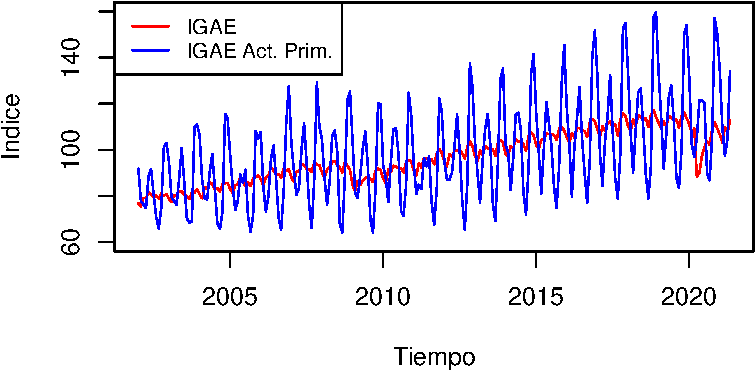
\includegraphics{index_files/figure-pdf/fig-fig1-1.pdf}

}

\end{figure}%

\subsection{b) Ejemplos y aplicaciones de las Series de
Tiempo}\label{b-ejemplos-y-aplicaciones-de-las-series-de-tiempo}

Un primer ejemplo que puede ilustrar la presencia de los dos tipos de
enfoques antes mencionadas es la Figura Figura~\ref{fig-fig1}. En esta
figura se muestra la evolución del Indicador Global de la Actividad
Económica (IGAE) en su versión global o del total de la economía y en su
versión únicamente para las actividades primarias entre enero de 2002 y
mayo de 2021.

Como se puede observar, el IGAE del total de la economía muestra,
principalmente, que el enfoque del tiempo es más relevante. Es decir,
que existe cierta persistencia en el indicador, lo que significa que la
economía crece en razón del crecimiento reportado en periodos pasados.
No obstante, lo que no podemos reconocer es que los eventos futuros
tienen un efecto en el desempeño de la economía hoy día. Así, no es
común observar cambios abruptos del indicador, salvo por la crisis
global de 2008 y la reciente crisis causada por la Covid-19.

\begin{Shaded}
\begin{Highlighting}[]
\FunctionTok{plot}\NormalTok{(ICC, }\AttributeTok{type =} \StringTok{"l"}\NormalTok{, }\AttributeTok{lwd =} \DecValTok{1}\NormalTok{, }\AttributeTok{col =} \StringTok{"red"}\NormalTok{, }\AttributeTok{ylab =} \StringTok{"Indice"}\NormalTok{, }\AttributeTok{xlab =} \StringTok{"Tiempo"}\NormalTok{, }\AttributeTok{ylim =} \FunctionTok{c}\NormalTok{(}\DecValTok{29}\NormalTok{, }\DecValTok{50}\NormalTok{))}
\CommentTok{\# Comando que indica a R que sin borrar la grafica anterior, grafique la siguiente.}
\FunctionTok{par}\NormalTok{(}\AttributeTok{new =}\NormalTok{ T)}
\CommentTok{\# Indice ??Como considera usted la situacion economica del pais hoy en dia comparada con la de hace 12 meses?, base enero 2003}
\FunctionTok{plot}\NormalTok{(ICC\_LAG, }\AttributeTok{type =} \StringTok{"l"}\NormalTok{, }\AttributeTok{lwd =} \DecValTok{1}\NormalTok{, }\AttributeTok{col =} \StringTok{"blue"}\NormalTok{, }\AttributeTok{ylab =} \StringTok{"Indice"}\NormalTok{, }\AttributeTok{xlab =} \StringTok{"Tiempo"}\NormalTok{, }\AttributeTok{ylim =} \FunctionTok{c}\NormalTok{(}\DecValTok{29}\NormalTok{,}\DecValTok{50}\NormalTok{))}
\CommentTok{\# Leyenda}
\FunctionTok{legend}\NormalTok{(}\StringTok{"bottomleft"}\NormalTok{, }\FunctionTok{c}\NormalTok{(}\StringTok{"ICC"}\NormalTok{,}\StringTok{"ICC lag"}\NormalTok{), }\AttributeTok{cex =} \FloatTok{0.8}\NormalTok{, }\AttributeTok{lty =} \DecValTok{1}\SpecialCharTok{:}\DecValTok{1}\NormalTok{, }\AttributeTok{col =} \FunctionTok{c}\NormalTok{(}\StringTok{"red"}\NormalTok{, }\StringTok{"blue"}\NormalTok{))}
\FunctionTok{par}\NormalTok{(}\AttributeTok{new =}\NormalTok{ F)}
\end{Highlighting}
\end{Shaded}

\begin{figure}[H]

\caption{\label{fig-fig2}índice de Confianza del Consumidor (ICC):
General y resultado de ¿Cómo considera usted la situación economica del
país hoy en día comparada con la de hace 12 meses? (puntos),
Ene.2002-may.2021}

\centering{

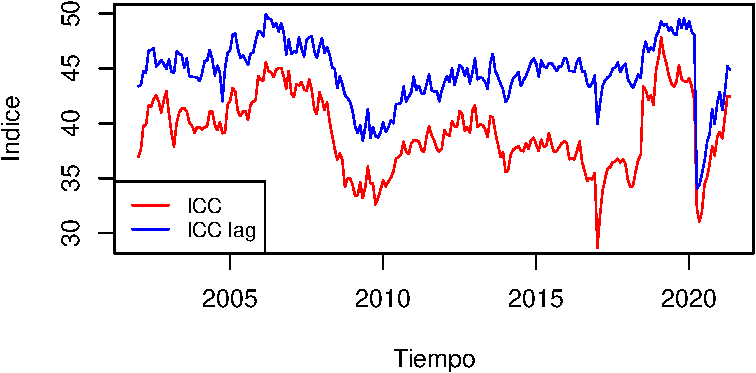
\includegraphics{index_files/figure-pdf/fig-fig2-1.pdf}

}

\end{figure}%

Por el contrario, el IGAE de las actividades primarias muestra una
presencia significativa de la importancia de la frecuencia. No pasa
desapercibido que existen muchos ciclos en la evolución del indicador.
Algo que suena común en las actividades primarias, cuya producción
depende de eventos que son ciclícos agrícolas asociados con el clima u
otros factores determinantes de la oferta de productos agrícolas. Otro
factor que puede incluir en el indicador son elementos de demanda, más
que los de oferta. Por ejemplo, el consumo de alimentos típicos de
algunas temporadas del año.

Como segundo ejemplo, en la Figura Figura~\ref{fig-fig2} se ilustra la
evolución reciente del índice de Confianza del Consumidor (ICC) en dos
de sus versiones: i) el Índice global y ii) el Índice de confianza de
los consumidores cuando estos consideran la situación actual en la
economía en relación el año anterior.

Destacamos que el ICC mide las expectativas de los consumidores en razón
de la información pasada y de la esperada, segun dichos consumidores.

\begin{Shaded}
\begin{Highlighting}[]
\CommentTok{\# Indice de Precios y Cotizaciones de la Bolsa Mexicana de Valores}
\FunctionTok{plot}\NormalTok{(IPC\_BMV, }\AttributeTok{type =} \StringTok{"l"}\NormalTok{, }\AttributeTok{lwd =} \DecValTok{1}\NormalTok{, }\AttributeTok{col =} \StringTok{"red"}\NormalTok{, }\AttributeTok{ylab =} \StringTok{"Indice"}\NormalTok{, }\AttributeTok{xlab =} \StringTok{"Tiempo"}\NormalTok{)}
\CommentTok{\# Tipo de Cambio para Solventar Obligaciones en Moneda Extranjera}
\FunctionTok{plot}\NormalTok{(TDC, }\AttributeTok{type =} \StringTok{"l"}\NormalTok{, }\AttributeTok{lwd =} \DecValTok{1}\NormalTok{, }\AttributeTok{col =} \StringTok{"blue"}\NormalTok{, }\AttributeTok{ylab =} \StringTok{"Pesos X Dolar"}\NormalTok{, }\AttributeTok{xlab =} \StringTok{"Tiempo"}\NormalTok{)}
\end{Highlighting}
\end{Shaded}

\begin{figure}

\caption{\label{fig-fig3}índice de Precios y Cotizaciones de la Bolsa
Mexicana de Valores (Panel Derecho) y Tipo de Cambio para Solventar
Obligaciones en Moneda Extranjera, pesos por dólar (Panel izquierdo),
Ene.2002-May.2021}

\begin{minipage}{0.50\linewidth}

\subcaption{\label{fig-fig3-1}Indice de Precios y Cotizaciones BMV}

\centering{

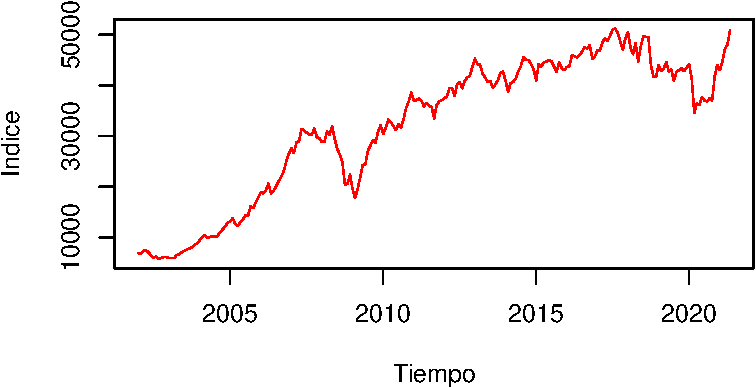
\includegraphics{index_files/figure-pdf/fig-fig3-1.pdf}

}

\end{minipage}%
%
\begin{minipage}{0.50\linewidth}

\subcaption{\label{fig-fig3-2}Tipo de Cambio}

\centering{

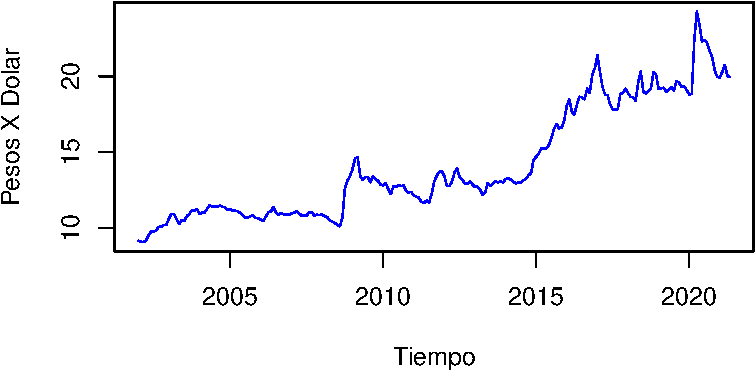
\includegraphics{index_files/figure-pdf/fig-fig3-2.pdf}

}

\end{minipage}%

\end{figure}%

Así, es probable que las dos series de tiempo exhiban un gran peso para
los eventos pasados, pero a la vez, un componente -probablemente menor-
del componente de frecuencia. Esto último en razón de que los
consumidores suelen considerar en sus expectativas de consumo los
periodos cíclicos de la economía: temporadas navideñas, pagos de
colegiaturas, etc. Este segundo ejemplo también ilustra que la confianza
del consumidor no necesariamente está directamente correlacionada con el
desempeño de la economía.

Como tercer ejemplo se muestra la evolución de dos series. La Figura
Figura~\ref{fig-fig3} ilustra el comportamiento reciente de dos
indicadores que son referencia para los inversionistas. Por un lado, se
ubica el índice de Precios y Cotizaciones de la BMV (IPC), el cuál
refleja el valor de las acciones de empresas que cotizan en la BMV y el
volumen de acciones comercializadas, en conjunto. De esta forma, se ha
interpretado que el IPC refleja el rendimiento del capital promedio
invertido en las empresas que cotizan en la BMV.

Por otro lado, en la Figura Figura~\ref{fig-fig3} se presenta la
evolución del Tipo de Cambio (TDC)\{indicador financiero que se suele
utilizar como medio de reserva de valor. Esto, en razón de que el TDC es
conocido como un instrumento que en momentos de crisis toma valores
contraciclicos de la economía mexicana. No obstante, ambos indicadores
no son comparables. Para hacerlos comparbles en la Figura
Figura~\ref{fig-fig4} se presentan en versión índice con una base en el
primer mes de la muestra.

\begin{Shaded}
\begin{Highlighting}[]
\NormalTok{IPC\_BMV\_I }\OtherTok{\textless{}{-}} \DecValTok{100}\SpecialCharTok{*}\NormalTok{IPC\_BMV}\SpecialCharTok{/}\NormalTok{IPC\_BMV[}\DecValTok{1}\NormalTok{]}
\NormalTok{TDC\_I }\OtherTok{\textless{}{-}} \DecValTok{100}\SpecialCharTok{*}\NormalTok{TDC}\SpecialCharTok{/}\NormalTok{TDC[}\DecValTok{1}\NormalTok{]}
\CommentTok{\# Indice del indice de Precios y Cotizaciones de la Bolsa Mexicana de Valores}
\FunctionTok{plot}\NormalTok{(IPC\_BMV\_I, }\AttributeTok{type =} \StringTok{"l"}\NormalTok{, }\AttributeTok{lwd =} \DecValTok{1}\NormalTok{, }\AttributeTok{col =} \StringTok{"red"}\NormalTok{, }\AttributeTok{ylab =} \StringTok{"Indice"}\NormalTok{, }\AttributeTok{xlab =} \StringTok{"Tiempo"}\NormalTok{, }\AttributeTok{ylim =} \FunctionTok{c}\NormalTok{(}\DecValTok{80}\NormalTok{,}\DecValTok{740}\NormalTok{))}
\CommentTok{\# Comando que indica a R que sin borrar la grafica anterior, grafique la siguiente.}
\FunctionTok{par}\NormalTok{(}\AttributeTok{new =}\NormalTok{ T)}
\CommentTok{\# Indice del Tipo de Cambio para Solventar Obligaciones en Moneda Extranjera}
\FunctionTok{plot}\NormalTok{(TDC\_I, }\AttributeTok{type =} \StringTok{"l"}\NormalTok{, }\AttributeTok{lwd =} \DecValTok{1}\NormalTok{, }\AttributeTok{col =} \StringTok{"blue"}\NormalTok{, }\AttributeTok{ylab =} \StringTok{"Indice"}\NormalTok{, }\AttributeTok{xlab =} \StringTok{"Tiempo"}\NormalTok{, }\AttributeTok{ylim =} \FunctionTok{c}\NormalTok{(}\DecValTok{80}\NormalTok{,}\DecValTok{740}\NormalTok{))}
\CommentTok{\# Leyenda}
\FunctionTok{legend}\NormalTok{(}\StringTok{"topleft"}\NormalTok{, }\FunctionTok{c}\NormalTok{(}\StringTok{"Indice del IPC"}\NormalTok{,}\StringTok{"Indice del TDC"}\NormalTok{), }\AttributeTok{cex =} \FloatTok{0.8}\NormalTok{, }\AttributeTok{lty =} \DecValTok{1}\SpecialCharTok{:}\DecValTok{1}\NormalTok{, }\AttributeTok{col =} \FunctionTok{c}\NormalTok{(}\StringTok{"red"}\NormalTok{, }\StringTok{"blue"}\NormalTok{))}
\FunctionTok{par}\NormalTok{(}\AttributeTok{new =}\NormalTok{ F)}
\end{Highlighting}
\end{Shaded}

\begin{figure}[H]

\caption{\label{fig-fig4}Índice del índice de Precios y Cotizaciones de
la Bolsa Mexicana de Valores (Panel Derecho) e Índice del Tipo de Cambio
para Solventar Obligaciones en Moneda Extranjera (ambos enero de 2002 =
100), pesos por dólar (Panel izquierdo), Ene.2002-May.2021}

\centering{

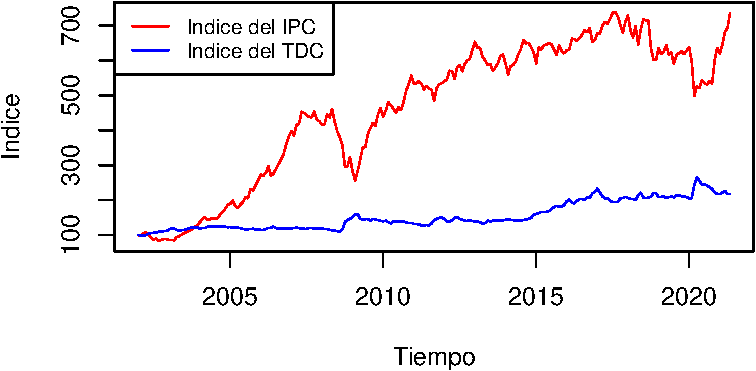
\includegraphics{index_files/figure-pdf/fig-fig4-1.pdf}

}

\end{figure}%

En la perspectiva de la Figura Figura~\ref{fig-fig4} se puede apreciar
que el TDC no es tan rentable, ya que una inversión en la BMV mediante
el IPC, en el largo plazo, muestra más redimientos. Asimismo, la Figura
Figura~\ref{fig-fig4}) ilustra que en ambas series se observa un dominio
de la condición de tiempo y no uno de frecuencia. Es decir, tanto el IPC
como el TDC no responden a condiciones como ciclos o temporadas que si
son observables en actividades económicas como las primarias.

Finalmente, la Figura Figura~\ref{fig-fig5} ilustra un característica
que también resulta de gran interés en el análisis de series de tiempo:
los datos de alta frecuencia y de comportamiento no regular. Como se
puede observar, en la Figura Figura~\ref{fig-fig5} se muestran las
diferencias logarítmicas de las series de IGAE de la actividad total, el
IPC y el TDC.

\begin{Shaded}
\begin{Highlighting}[]
\CommentTok{\# Indicador Global de la Actividad Econimica, base 2008}
\FunctionTok{plot}\NormalTok{(}\FunctionTok{diff}\NormalTok{(}\FunctionTok{log}\NormalTok{(IGAE\_2013), }\AttributeTok{lag =} \DecValTok{1}\NormalTok{), }\AttributeTok{type =} \StringTok{"l"}\NormalTok{, }\AttributeTok{lwd =} \DecValTok{1}\NormalTok{, }\AttributeTok{col =} \StringTok{"red"}\NormalTok{, }\AttributeTok{ylab =} \StringTok{"Var. \%"}\NormalTok{, }\AttributeTok{xlab =} \StringTok{"Tiempo"}\NormalTok{)}
\CommentTok{\# Indice de Precios y Cotizaciones de la Bolsa Mexicana de Valores}
\FunctionTok{plot}\NormalTok{(}\FunctionTok{diff}\NormalTok{(}\FunctionTok{log}\NormalTok{(IPC\_BMV), }\AttributeTok{lag =} \DecValTok{1}\NormalTok{), }\AttributeTok{type =} \StringTok{"l"}\NormalTok{, }\AttributeTok{lwd =} \DecValTok{1}\NormalTok{, }\AttributeTok{col =} \StringTok{"red"}\NormalTok{, }\AttributeTok{ylab =} \StringTok{"Var. \%"}\NormalTok{, }\AttributeTok{xlab =} \StringTok{"Tiempo"}\NormalTok{)}
\CommentTok{\# Tipo de Cambio para Solventar Obligaciones en Moneda Extranjera}
\FunctionTok{plot}\NormalTok{(}\FunctionTok{diff}\NormalTok{(}\FunctionTok{log}\NormalTok{(TDC), }\AttributeTok{lag =} \DecValTok{1}\NormalTok{), }\AttributeTok{type =} \StringTok{"l"}\NormalTok{, }\AttributeTok{lwd =} \DecValTok{1}\NormalTok{, }\AttributeTok{col =} \StringTok{"blue"}\NormalTok{, }\AttributeTok{ylab =} \StringTok{"Pesos X Dolar"}\NormalTok{, }\AttributeTok{xlab =} \StringTok{"Tiempo"}\NormalTok{)}
\end{Highlighting}
\end{Shaded}

\begin{figure}

\caption{\label{fig-fig5}Tasas de Crecimiento mensuales (diferencias
logarítmicas) de Indicador Global de la Actividad Económica, Índice de
Precios y Cotizaciones de la Bolsa Mexicana de Valores (Panel Derecho) y
Tipo de Cambio para Solventar Obligaciones en Moneda Extranjera,
Ene.2002-May.2021}

\begin{minipage}{\linewidth}

\subcaption{\label{fig-fig5-1}Indicador Global de la Actividad
Economica}

\centering{

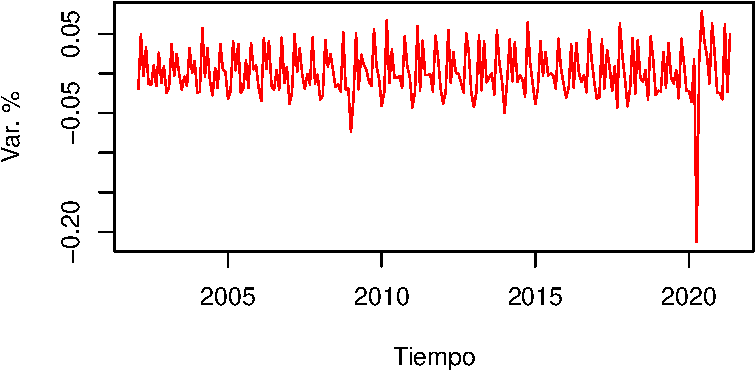
\includegraphics{index_files/figure-pdf/fig-fig5-1.pdf}

}

\end{minipage}%
\newline
\begin{minipage}{\linewidth}

\subcaption{\label{fig-fig5-2}Indice de Precios y Cotizaciones BMV}

\centering{

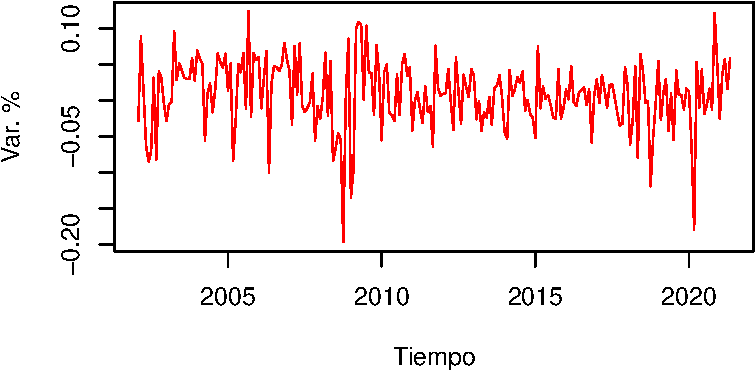
\includegraphics{index_files/figure-pdf/fig-fig5-2.pdf}

}

\end{minipage}%
\newline
\begin{minipage}{\linewidth}

\subcaption{\label{fig-fig5-3}Tipo de Cambio}

\centering{

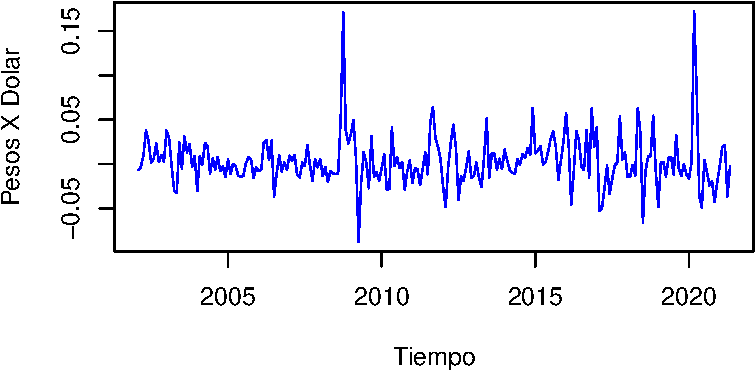
\includegraphics{index_files/figure-pdf/fig-fig5-3.pdf}

}

\end{minipage}%

\end{figure}%

Dichas diferencia se pueden interpretar como una tasa de crecimiento de
las series por las siguientes razones. Consideremos una serie de tiempo
dada por \(y_t\), cuya versión logarítmica es \(ln(y_t)\). De esta
forma, la diferencia logarítmica esta dada por la ecuación
(Ecuación~\ref{eq-difflog}):

\begin{equation}\phantomsection\label{eq-difflog}{
\Delta ln(y*t) = ln(y_t) - ln(y*{t-1}) = ln \left( \frac{y*t}{y*{t-1}} \right)
}\end{equation}

Ahora bien, si retomamos la definición de tasa de crecimiento (TC) de
una serie de tiempo \(y_t\) entre el periodo \(t\) y \(t-1\) podemos
obtener que:

\begin{equation}\phantomsection\label{eq-TC}{
TC = \frac{y*t - y*{t-1}}{y*{t-1}} = \frac{y_t}{y*{t-1}} - 1
}\end{equation}

De esta forma, si tomamos el logarítmo de la expresión de la ecuación
(Ecuación~\ref{eq-TC}) obtenemos la siguiente aproximación:

\begin{equation}\phantomsection\label{eq-TCDiffLog}{
\frac{y*t}{y*{t-1}} -1 \approx ln \left( \frac{y*t}{y*{t-1}} \right) = ln(y*t) - ln(y*{t-1})
}\end{equation}

La ecuación (Ecuación~\ref{eq-TCDiffLog}) es cierta cuando los valores
de \(y_t\) y \(y_{t-1}\) son muy parecidos, es decir, cuando las
variaciones no son tan abruptas. Otra forma de interpretar la ecuación
(Ecuación~\ref{eq-TCDiffLog}) es que para tasas de crecimiento pequeñas,
se puede utilizar como una buena aproximación a la diferencia
logarítmica mostrada en la ecuación (Ecuación~\ref{eq-difflog}).

En la Figura Figura~\ref{fig-fig5} se reportan las diferencias
logarítmicas del IGAE, IPC y TDC, todos, como una media de distitntos
tipos de redimientos. Es decir, podemos decir que un capitalista
promedio (suponiendo que solo puede invertir en la actividad económica,
en la bolsa o en el dólar), puede observar que le es más redituable en
función de sus preferencias.

Notése que la dinámica de las variaciones de cada una de las series es
significativamente diferente. Destaca que el TDC es una de las variables
que, en general, no muestra grandes cambios a lo largo del tiempo. No
obstante, se han observado cambios radicales, cuando menos en el año
2008. Lo anterior, son características que se han observado para el IPC.
En cambio, el IGAE muestra un comportamiento más estable o estacionario.


\printbibliography


\end{document}
